\section{Analysis}\label{sc:analysis}
Two verification problems were created in order to ensure
that the implementation of the rnucs-mesh workflow was correct.
These verification problems were constructed in a manner that
high energy interactions would occur.

\subsection{Verification Problem I}
\subsubsection{Geometry}
Verification problem I (shown in Figure \ref{TPI}) consists of a mercury rectangular prism that is 
22 cm x 44 cm x 186 cm. 
%
\begin{figure}[h!]
\begin{centering}
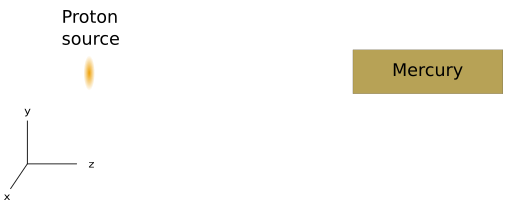
\includegraphics[width=0.60\linewidth]{../figs/mercury.png}
\caption{Planar view of Verification Problem I geometry, 22 cm  x 44 cm x 186 cm }
\label{TPI}
\end{centering}
\end{figure}
%
\subsubsection{Source}
The source was the same used in the Spallation Neutron Source (SNS). The source
is a proton sourcde with energy gaussian distribution centered around 1 GeV.
The source is located in the xy plane at z = -256.71 cm, where the distribution
of the x plane depends on the y location.
%
\subsubsection{Spatial Discretization}
Several superimposed meshes were laid over the verification problem.
The superimposed meshes were 1x1x1, 2x2x2, and 4x4x4.
The geometry was also split into 8 and 64 euqal pieces in order to
directly compare to the 2x2x2 and 4x4x4 mesh respectively.
A full workflow was run with the following configurations.
\begin{itemize}
\item Mercury cell
\item 1x1x1 uniformly distributed mesh superimposed on the whole problem
\item 2x2x2 uniformly distributed mesh superimposed on the whole problem
\item 4x4x4 uniformly distributed mesh superimposed on the whole problem
\item Geometry split into 8 equal pieces
\item Geometry split into 64 equal pieces
\end{itemize}
\subsubsection{Results}
A comparison between the radionuclide production collected in cell,
and meshes of sizes 1x1x1, 2x2x2, and 4x4x4. The mesh results were added
across all mesh volumes for a direct
comparison to the cell results. These are shown in Figure \ref{fig:1prod_cell_2x_4x}.
A similar comparison was done for the photon spectrum resulting from the activation
step. The results are shown in figure \ref{fig:1spec_cell_2x_4x}
\begin{figure}[h!]
 \begin{centering}
 \centering
 \begin{subfigure}[b]{.8\textwidth}
 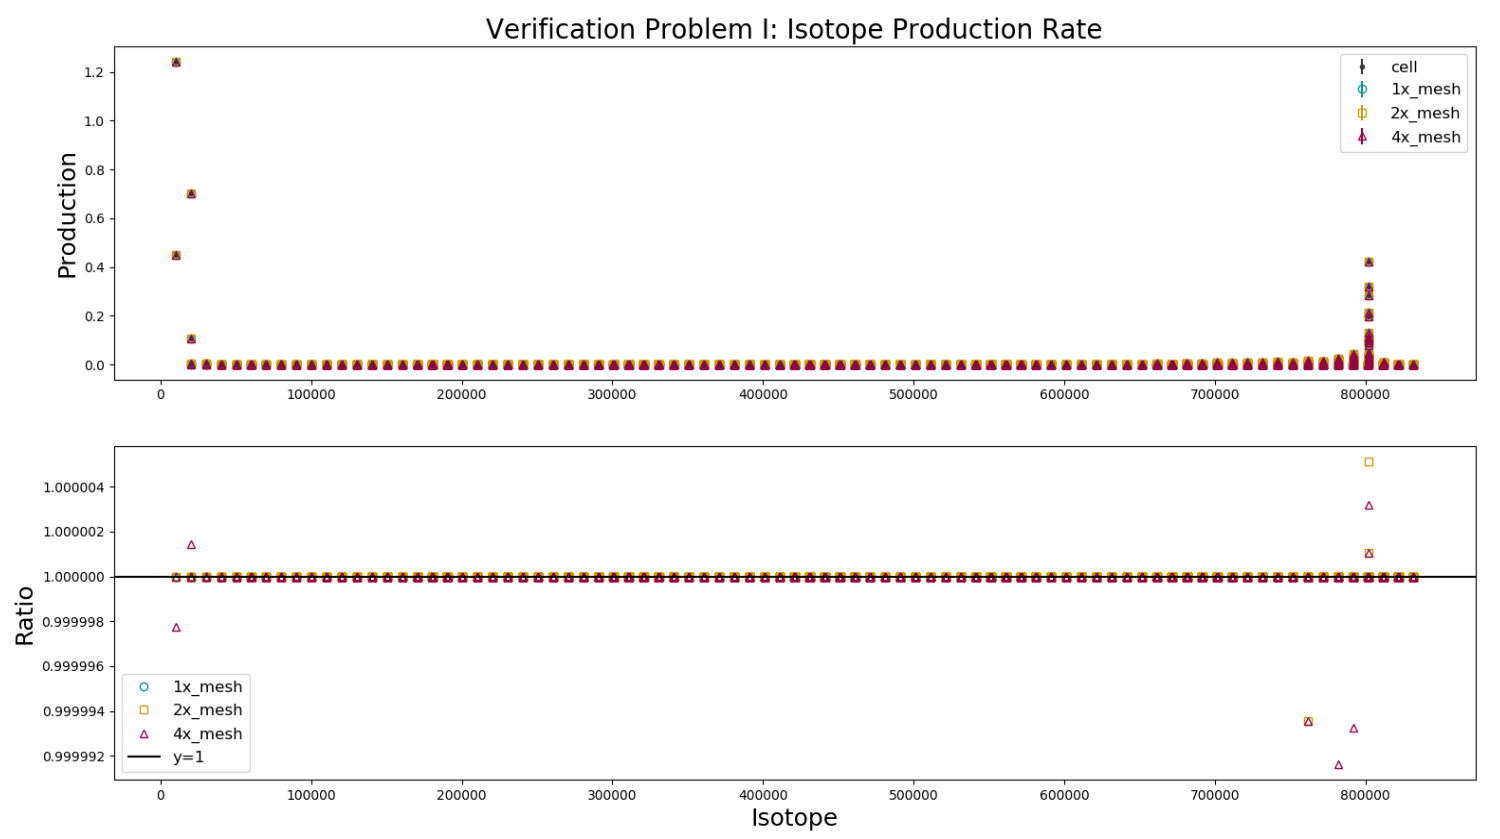
\includegraphics[width=0.99\linewidth,height=8cm]{../figs/toy_p1/prod_VPI_1x_2x_4x.png}
 \caption{Radionuclide production rates}
 \label{fig:1prod_cell_2x_4x}
 \end{subfigure}
 \hspace{0.05cm}
 %
 \begin{subfigure}[b]{.8\textwidth}
 \centering
 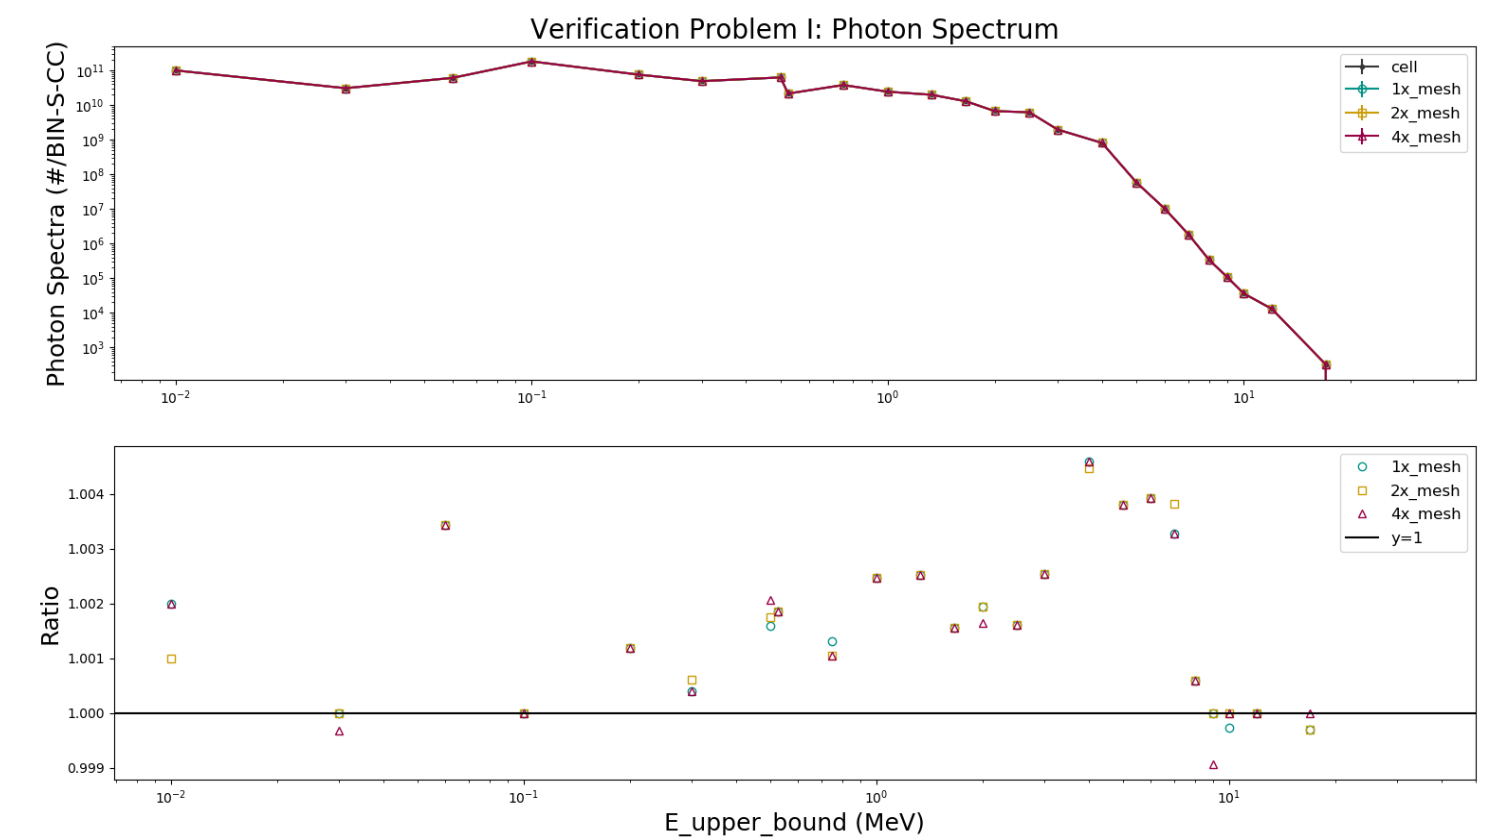
\includegraphics[width=.99\linewidth,height=8cm]{../figs/toy_p1/spec_VPI_1x_2x_4x.png}
 \caption{Photon emission rate at 1 minute decay }
 \label{fig:1spec_cell_2x_4x}
 \end{subfigure}
 \caption{Verification Problem I: Comparison between results for geometric cell, and different size meshes}
 \label{cell_2x_4x}
 \end{centering}
\end{figure}
%
A comparison between the results collected in a cell, 2x2x2 mesh, and
the geometry split into 8 equal pieces. The results for the radionuclide production
and the photon spectrum are shown in Figures \ref{fig:1prod_cell_2x} and
\ref{fig:1spec_cell_2x} respectively.
\begin{figure}[h!]
 \begin{centering}
 \centering
 \begin{subfigure}[b]{.8\textwidth}
 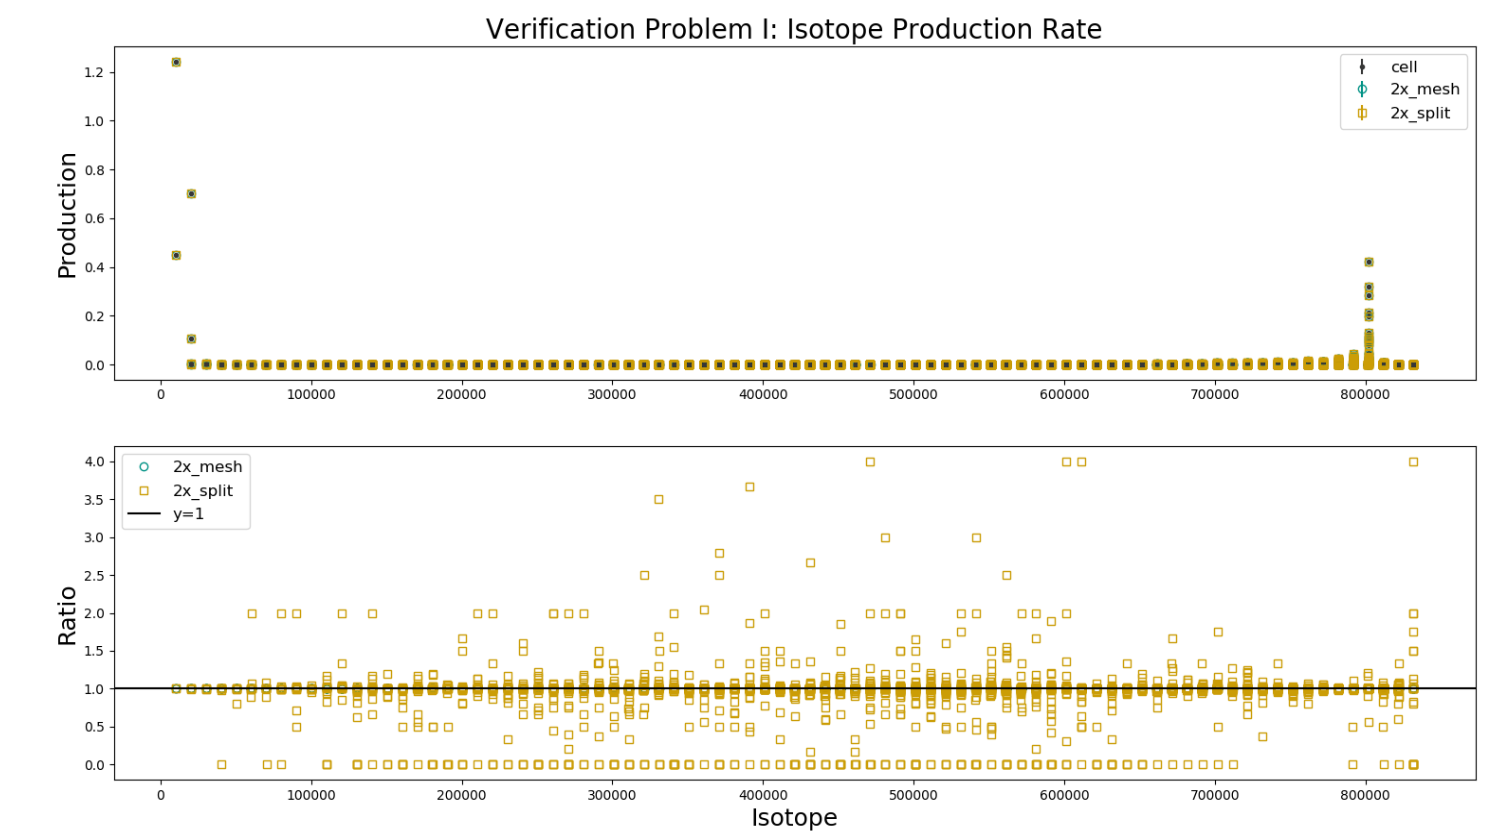
\includegraphics[width=0.99\linewidth,height=8cm]{../figs/toy_p1/prod_VPI_2x.png}
 \caption{Radionuclide production rates}
 \label{fig:1prod_cell_2x}
 \end{subfigure}
 \hspace{0.05cm}
 %
 \begin{subfigure}[b]{.8\textwidth}
 \centering
 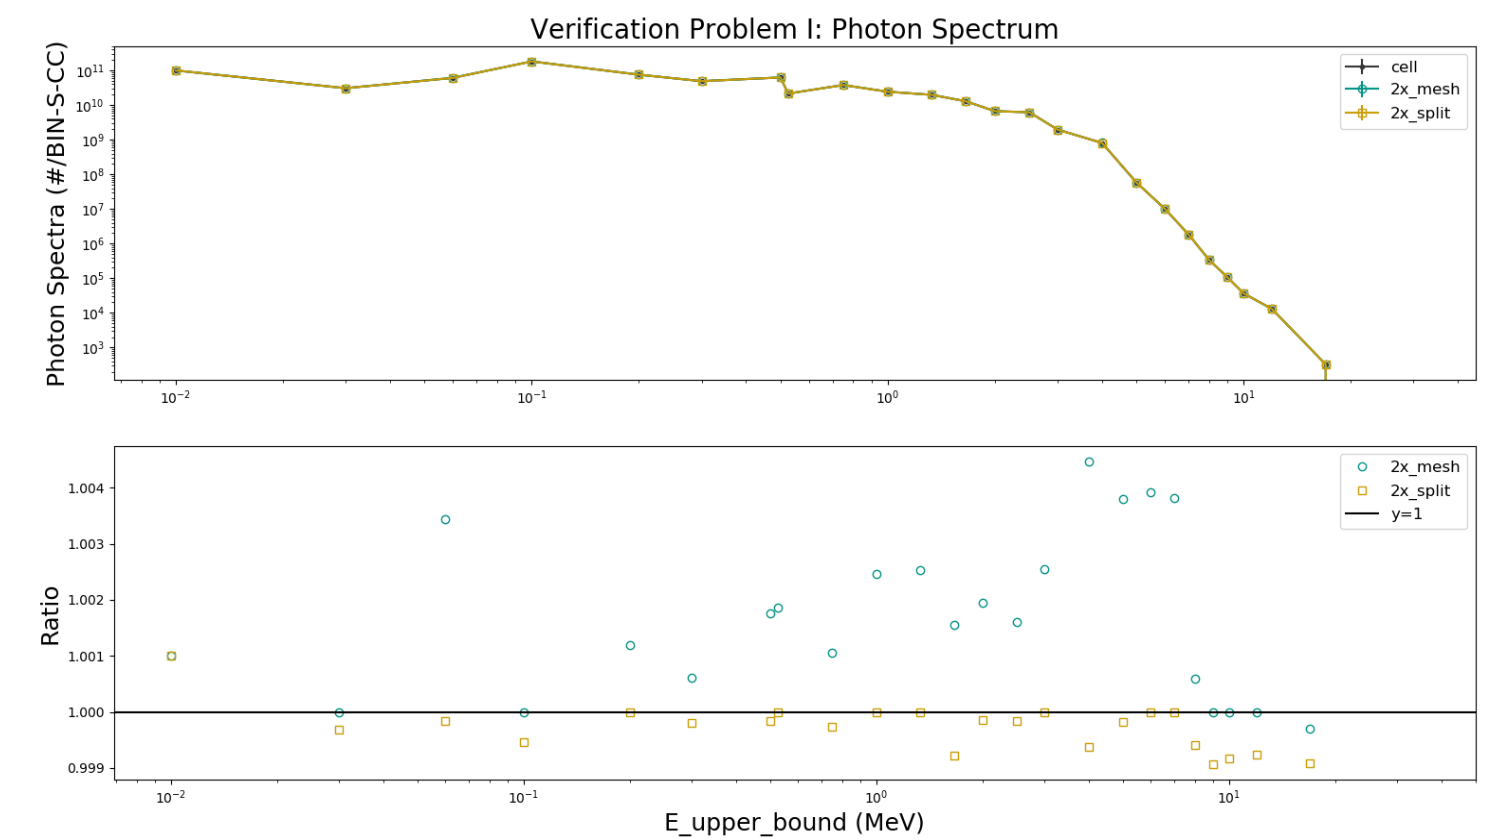
\includegraphics[width=.99\linewidth,height=8cm]{../figs/toy_p1/spec_VPI_2x.png}
 \caption{Photon emission rate at 1 minute decay }
 \label{fig:1spec_cell_2x}
 \end{subfigure}
 \caption{Verification Problem I: Comparison between results for geometric cell, and different size meshes}
 \label{fig:cell_2x}
 \end{centering}
\end{figure}
%
A similar comparison as the one above was performed with 4x4x4 mesh and
the geometry split into 64 equal parts. The results are shown in Figures
\ref{fig:1prod_cell_4x} and \ref{fig:1spec_cell_4x}.
\begin{figure}[h!]
 \begin{centering}
 \centering
 \begin{subfigure}[b]{.8\textwidth}
 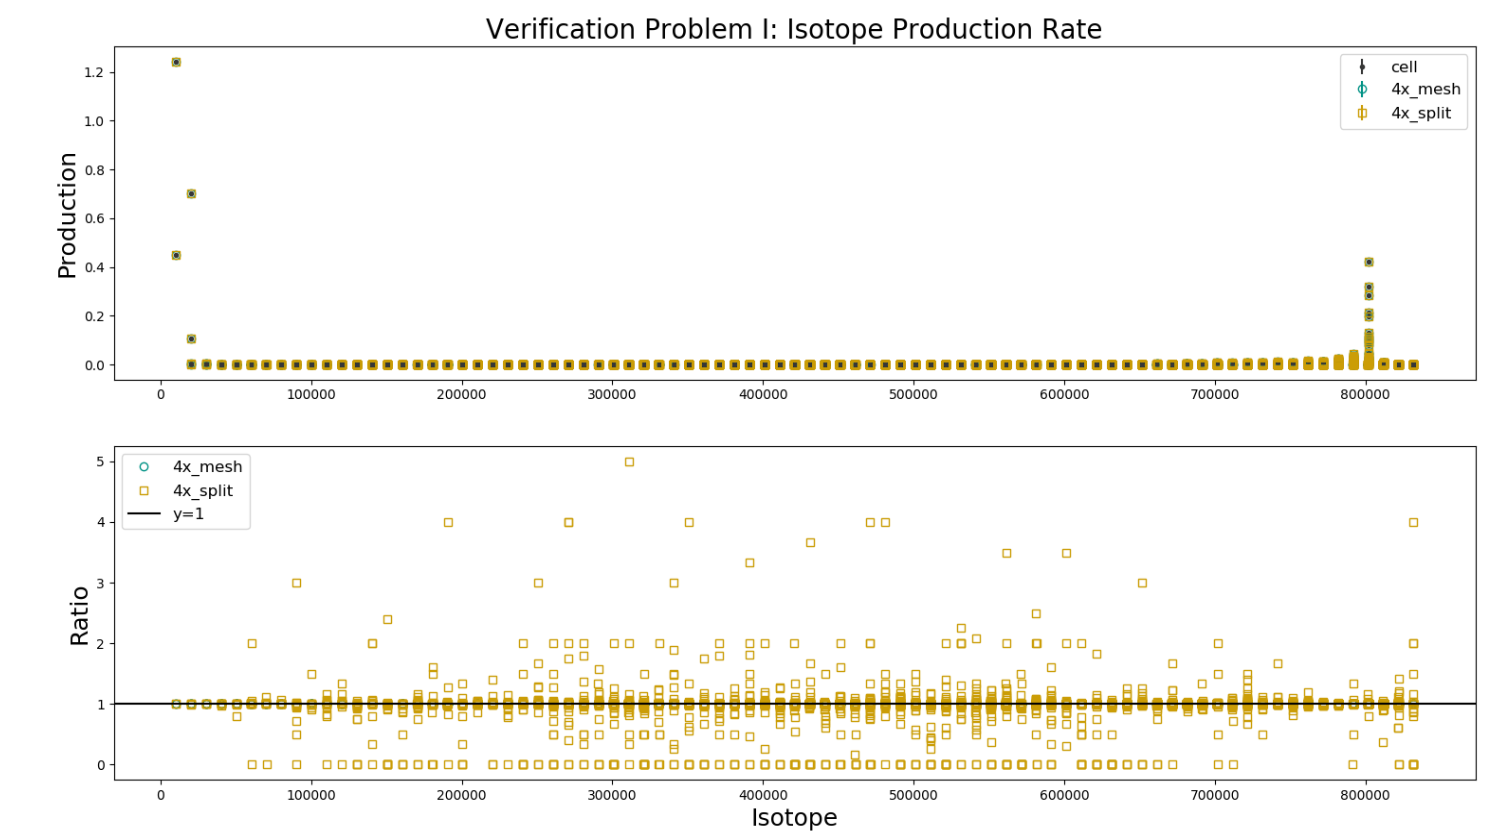
\includegraphics[width=0.99\linewidth,height=8cm]{../figs/toy_p1/prod_VPI_4x.png}
 \caption{Radionuclide production rates}
 \label{fig:1prod_cell_4x}
 \end{subfigure}
 \hspace{0.05cm}
 %
 \begin{subfigure}[b]{.8\textwidth}
 \centering
 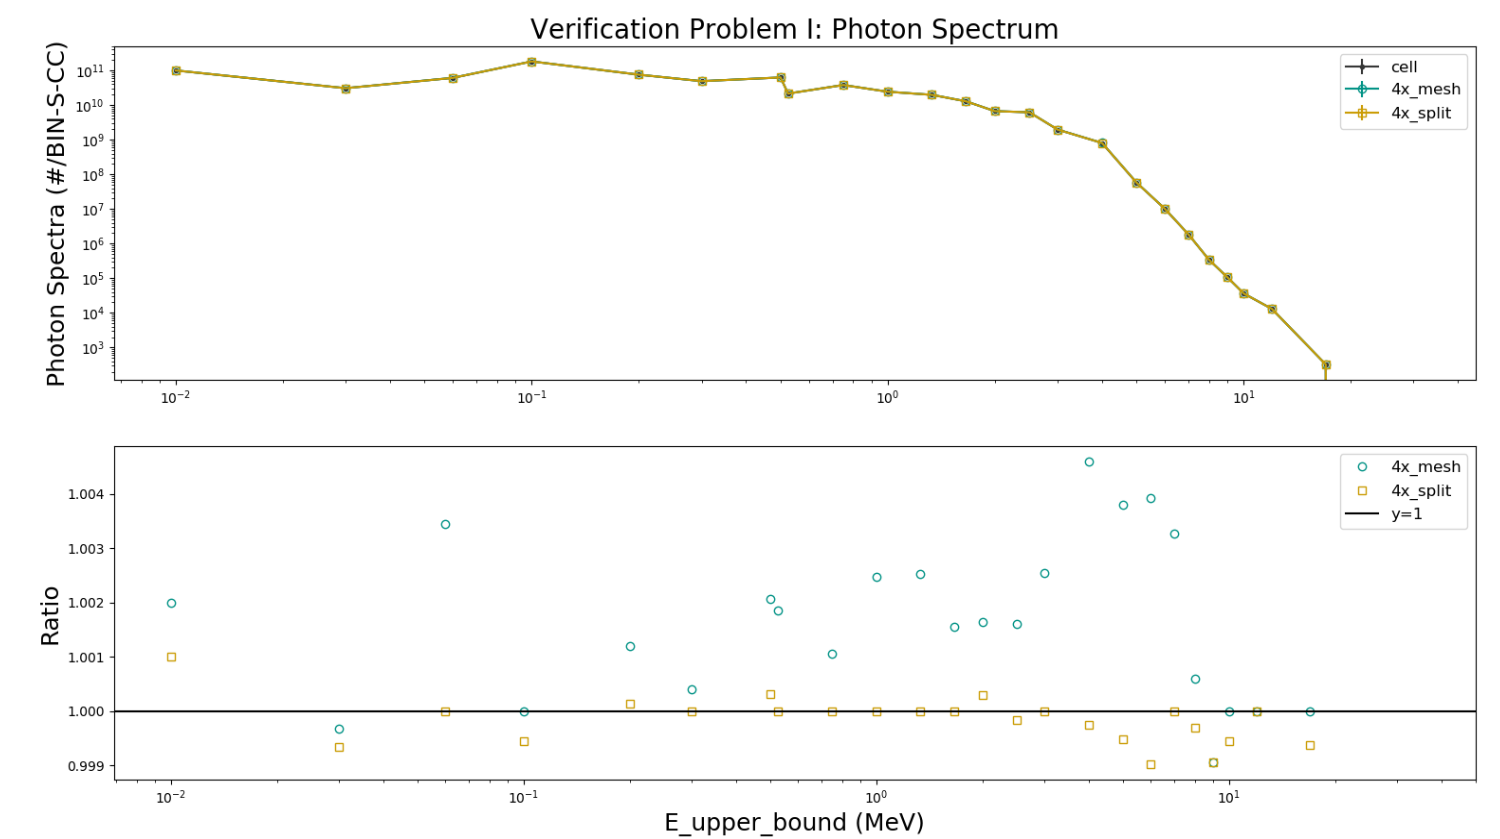
\includegraphics[width=.99\linewidth,height=8cm]{../figs/toy_p1/spec_VPI_4x.png}
 \caption{Photon emission rate at 1 minute decay }
 \label{fig:1spec_cell_4x}
 \end{subfigure}
 \caption{Verification Problem I: Comparison between results for geometric cell, and different size meshes}
 \label{fig:cell_4x}
 \end{centering}
\end{figure}

%%%%%%%%%%%%%%%%%%
\newpage
\subsection{Problem Description}
Two verification problems were identified to asses the correctness of the
rnucs-mesh workflow.

Verification problem II (shown in Figure \ref{TPII}) has a rectangular prism enclosing another rectangular
prism. 
The mercury cell has the same dimensions as those of verification problem I. The steel 
cell, which encloses the mercury, is double the size of the mercury cell. 
% Figure
% Figure
\begin{figure}[h!]
\begin{centering}
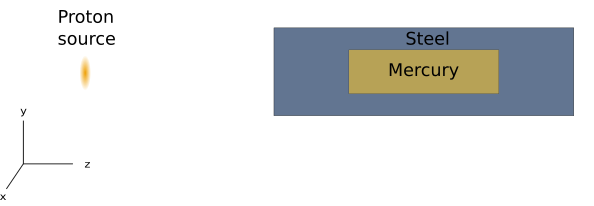
\includegraphics[width=0.70\linewidth]{../figs/mer_steel.png}
\caption{Planar view of Verification Problem II geometry, 44 cm x 88 cm x 372 cm }
\label{TPII}
\end{centering}
\end{figure}

Both verification problems have a source that models that of the
actual SNS systems. The source is a proton source with energy gaussian dritribution
around 1 GeV. The source is located in a distributed xy plane at z = -256.71 cm, 
where the distribution of the x plane denpends on the y location. 

\subsubsection{Spatial Discretization}
Several superimposed meshes were laid upon Verification Problem I and II. 
The superimposed meshes were 1x1x1, 2x2x2, and 4x4x4. Both verification problems
were also split into 8 equal pieces and 64 equal pieces creating a total of
six distint geometries including the originals. 
Splitting verification problem II into 8 equal cells required some material mixing. 
Each cell in this particular geometry was assigned a steel-mercury mixture
of 3:1. 
This splitting was done in order to compare to the mesh problems. 

\subsection{Workflow to Photon Emissions}
In order to generate the spectrum file, the following steps were carried out:
\begin{itemize}
\item Monte Carlo transport using MCNP 
\item Activation script was run to create the input files for CINDER and  run CINDER
\end{itemize}
A total of 12 problems were run, six for each verification problem. The runs were as follows:
\begin{itemize}
\item Cell rnucs. Mercury cell for Verification Problem I and Mercury and Steel cell for
Verification Problem II.
\item 1x1x1 uniformly distributed mesh superimposed on the whole problem
\item 2x2x2 uniformly distributed mesh superimposed on the whole problem
\item 4x4x4 uniformly distributed mesh superimposed on the whole problem
\item Geometry split into 8 equal pieces
\item Geometry split into 64 equal pieces
\end{itemize}
Each case was run with 1E6 history particles. 

\newpage
